\section{The \lhcb trigger}
\label{sec:lhcb:trig}

The trigger in \lhcb selects events which contain common signatures of heavy flavour hadron decays which are suitable for subsequent reconstruction. 
The trigger design is motivated by the infrequency of \bbbar production and also the small branching fraction of decays such as \BdToKstmm, which is of order $10^{-6}$. 
At the \lhc collision energy of 7\tev, the total cross-section of $pp$ interactions when single diffractive processes are included is 50\mbarn but 
the \bbbar cross-section in the \lhcb acceptance is around 75\mub~\cite{LHCb-PAPER-2011-003}.
%A second requirement is the difference between the  frequency of $pp$ interactions at \lhcb which is $\sim40\mhz$ for the proton bunch spacing of 50ns in 2011
 %and the output rate at which it is possible to write events to tape at $\sim4\khz$.
The trigger is required to reduce the event rate from about 10\mhz to an output rate of around 4\khz. %with a bunch spacing of 50\ns
The \lhcb trigger and its performance in 2011 is documented in Ref.~\cite{Aaij:2012me} and 
an illustration of the stages of the \lhcb trigger can be seen in Fig.~\ref{fig:lhcb:trigger}.
\begin{figure}
\centering
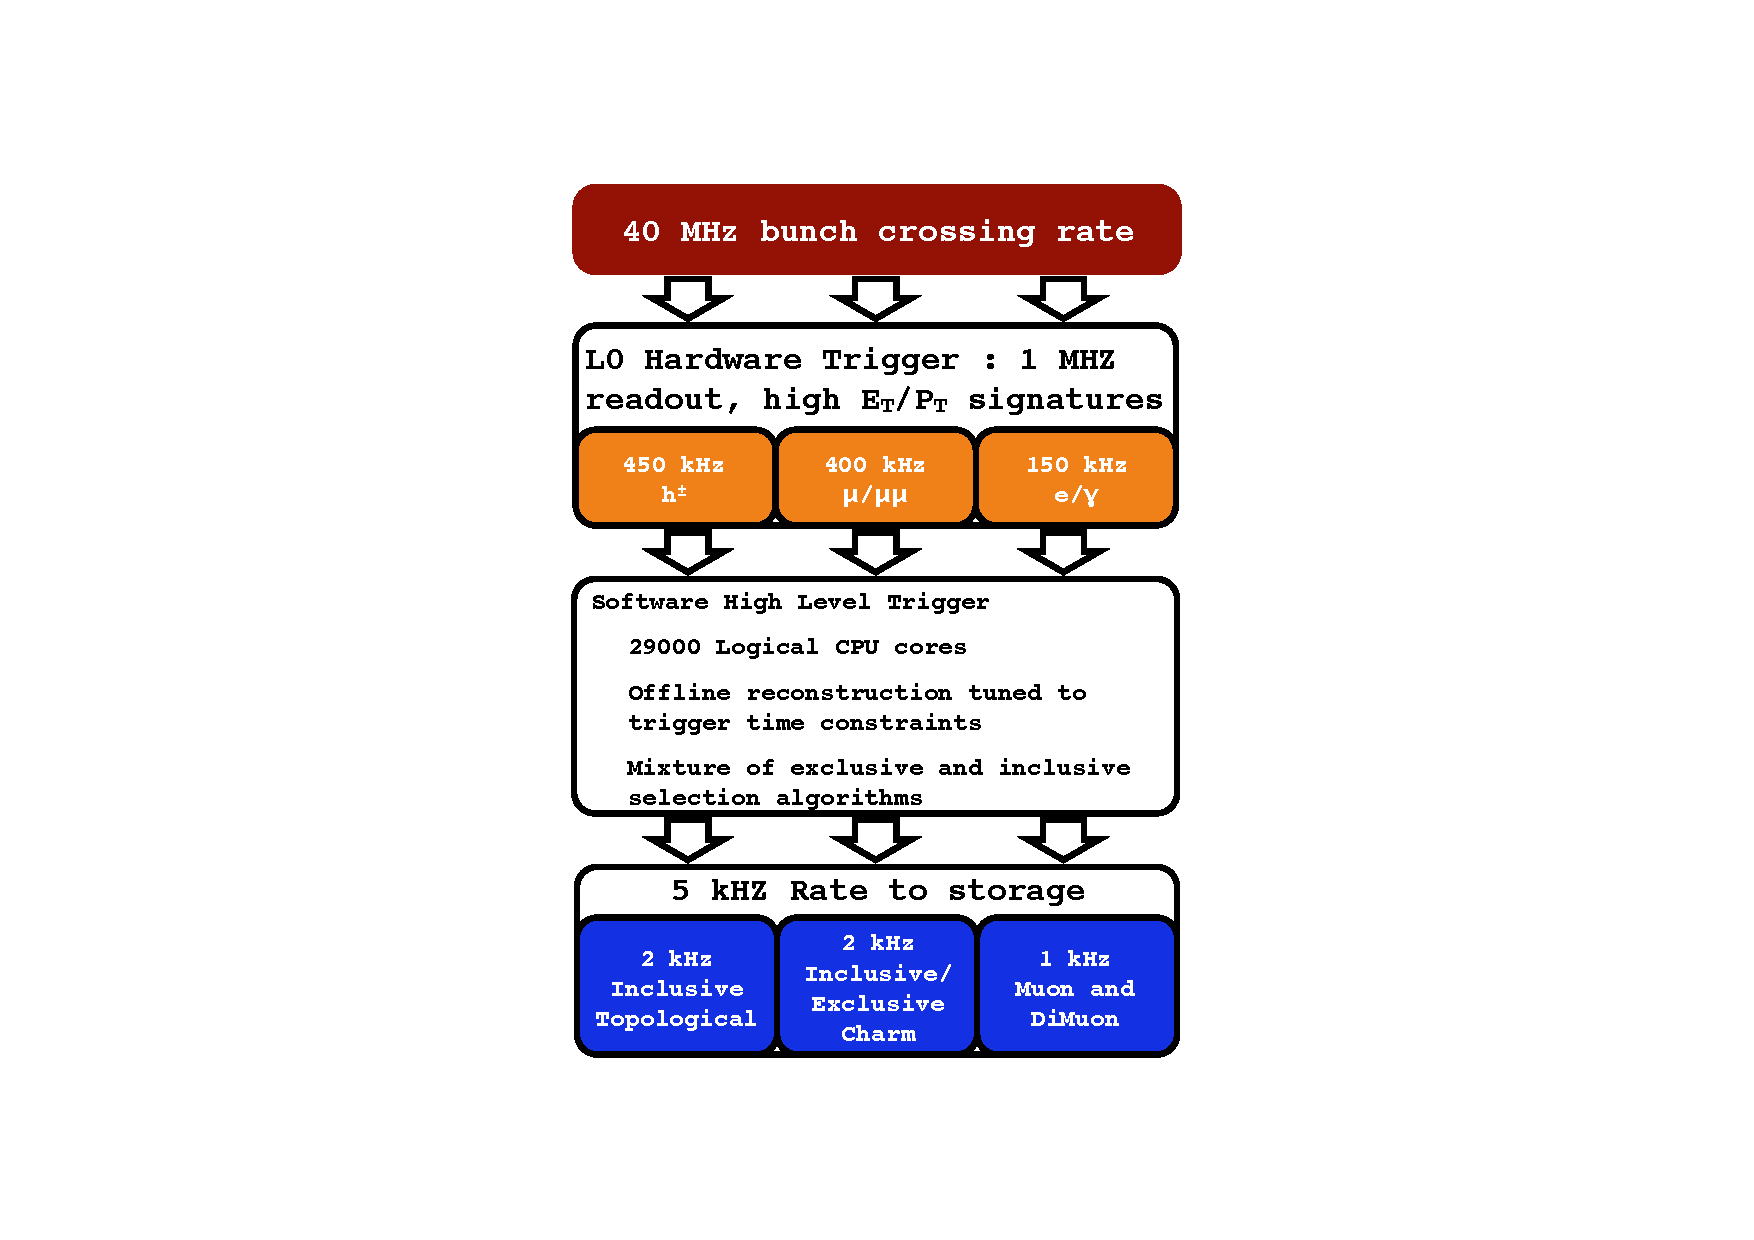
\includegraphics[width=0.88\columnwidth]{chapter3/figs/LHCb_Trigger_Plot.pdf}
\caption[The \lhcb trigger system.]
{An illustration of the \lhcb trigger system showing the two distinct stages with the rate of data input
and output and the three main trigger line categories~\cite{Aaij:2012me}.~\label{fig:lhcb:trigger}}
\end{figure}
The \lhcb trigger consists of two stages, a hardware stage called Level 0 (\lzero) and a software stage, the high level trigger (\hlt).
This separation and the further separation of the \hlt into two sub-stages is due to the different timing required to process the information
and the amount of information available within the time limit for the trigger stage.

\subsection{The hardware trigger}

The \lzero trigger is a hardware trigger because it is required to accept or reject events faster than the time that the sub-detectors can buffer the data.
The \lzero trigger reduces the incoming rate from 10\mhz to 1\mhz by selecting events with basic characteristics of \bquark-hadron events.
These characteristics are either the presence of muons with high transverse momentum (\pt), \lzmuon, or the presence of large energy deposits in the calorimeters, L0Calo.
The \lzmuon channel triggers on high \pt muons by assigning each quadrant of the muon stations to a different processor.
The \pt of the muon is calculated through the information from the the \Mone and \Mtwo stations and an 
event is triggered if there is one high \pt muon passing through the same quadrant of all five muon stations.

\subsection{The software trigger}

Once events are selected by the \lzero trigger, they pass from the detector electronics to a batch system of processors called the Event Filter 
Farm (EFF). 
There are 29,000 instances of the \hlt running as software processes on the EFF,
 where they are processed by the \hlt algorithms to decide whether the event contains enough interesting information and should be written to tape. 
Event-by-event, the \hlt is required to make a decision in under 30\ms.

The first stage of the \hlt (\hltone) performs basic particle track reconstruction. 
The \hltotrack trigger line triggers on events which pass any \lzero decision that contain one prominent track with a high momentum and a high impact parameter.
The impact parameter (IP) is defined as the distance between the vector of the reconstructed track and the point of the primary vertex.
Alternatively, if the event fired the \lzmuon trigger the muon candidate is reconstructed.
The \hltomuon trigger selects the event if the muon candidate had a momentum above 6\gevc.
%The \hltone reduces the rate sufficiently to allow high momentum tracks to be reconstructed and processed by the second state of the software trigger, \hlttwo.

The second software trigger (\hlttwo) performs further reconstruction of tracks in order to filter events down to a final output rate of around 4\khz.
For the processing of data in 2011, the \hlttwo was re-written in order to cope with conditions different to the design requirements.
The main trigger  in \hlttwo is a `topological trigger` which is designed to select partially reconstructed \bquark-hadron decays from combinations of 
2, 3, or 4 tracks and select on properties of the n-body combination.
There are two other triggers which are exclusive muon triggers that select good quality high momentum muons 
with a significant impact parameter and a large \pt, similar to the \hltomuon trigger.
The development of the \hlttwo is described in Section~\ref{sec:lhcb:trigdev}.



